\documentclass[a4paper,12pt]{article}

% Packages
\usepackage[utf8]{inputenc}
\usepackage[T1]{fontenc}
\usepackage{geometry}
\usepackage{graphicx}
\usepackage[hidelinks]{hyperref}
\usepackage{amsmath}
\usepackage{amsthm}
\usepackage{amssymb}
\usepackage{bbm}
\usepackage{float}
\usepackage{booktabs}
\usepackage{siunitx}
\usepackage{comment}
\usepackage{subcaption}
\usepackage{minted}
\usepackage{authblk}


\usepackage[backend=biber,style=numeric,citestyle=numeric]{biblatex}
\addbibresource{references.bib}

\theoremstyle{definition}
\newtheorem{theorem}{Theorem}
\newtheorem{definition}{Definition}
\newtheorem{remark}{Remark}

% Page setup
\geometry{margin=1in}

\begin{document}

\begin{titlepage}
    \centering
    {\Large Sorbonne Université \\ M2 Statistiques}
    
    \vspace{3cm}

    {\Huge \textbf{Synthetic turbulence generation using statistical methods}}

    \vspace{3cm}

    % Authors manually
    {\Large Samy Braik \\[0.3cm]
    Supervisor: Aurélien Larcher\textsuperscript{1}, Jonathan Viquerat\textsuperscript{1}, Fabien Duval\textsuperscript{2}, Aubin Brunel\textsuperscript{2} \\[0.3cm]
    \textsuperscript{1}CEMEF, Mines Paris – PSL \\ 
    \textsuperscript{2}ANSR}

    \vfill

    % Logos
    \begin{minipage}{0.45\textwidth}
        \centering
        
\includegraphics[width=\textwidth]{illustrations/minesparis.png}
    \end{minipage}
    \hfill
    \begin{minipage}{0.45\textwidth}
        \centering
        
\includegraphics[width=\textwidth]{illustrations/logo_cemef.jpg}
    \end{minipage}

    \vfill

    {\Large \today}
\end{titlepage}





\newpage
\tableofcontents
\newpage

\section{Introduction}
Turbulence describes the unpredictable and complex motion of a fluid, characterized by chaotic vortices spanning a wide range of scales. The behavior of a fluid is commonly quantified by the Reynolds number (Re): the higher the Re, the more turbulent the flow. Turbulence plays a crucial role in many natural and engineering systems, from atmospheric flows to industrial mixing, and its multiscale nature makes it challenging to model accurately.

In this work, we focus on an idealized type of turbulence known as Homogeneous and Isotropic Turbulence (HIT). HIT is widely used in fundamental turbulence studies because it isolates the intrinsic statistical properties of turbulence without the complications of boundaries or anisotropies. This flow exhibits two key properties: it is homogeneous, meaning statistical quantities (mean, variance, correlation functions) are independent of spatial position, and isotropic, meaning these statistics remain invariant under rotations or reflections of the coordinate system. These characteristics make HIT a convenient test case for validating computational models of turbulent velocity fields.


\begin{figure}[H]
    \centering
    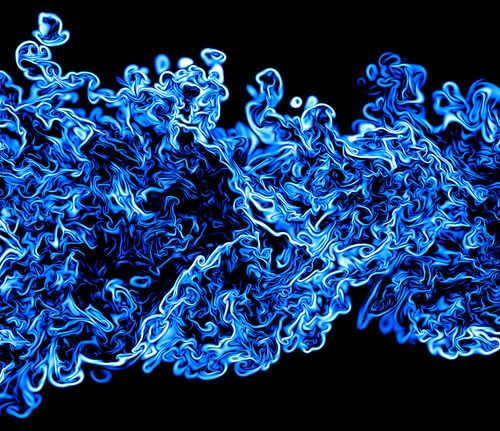
\includegraphics[width=0.5\textwidth]{illustrations/TurbulenceExample.jpg}
    \caption{Slice through the field of the scalar dissipation reveals the small-scale structure of turbulence from CNRS UMR 6614 CORIA and JSC}
\end{figure}


When the goal is to use statistical methods to produce turbulent velocity field two paths are worth considering. The first one is to simply use a statistical method that generate the velocity field directly. This is done in \cite{Yousif_Yu_Lim_2022},\cite{wang2025fourierflowfrequencyawareflowmatching} or \cite{parikh2025conditionalflowmatchinggenerative}. \\
Here, generative models seem the most suitable. Two major difficulties could be encountered, the huge cost and the poor generalization of these approaches. Indeed, in order to train such a model, there is a need for highly resolved turbulence usually produced with Direct Numerical Simulation (DNS) which are costly numerical methods. Apart from that, there is the natural drawback of the method itself that can't be sidelined. The poor generalization of the method stem from the fact that usually, the models are trained on fields with a specific Reynolds number which leads to poor robustness if the turbulence parameters are changed. \\
The other path would be to start from an already existent method. For example in the case of Reynolds-averaged Navier–Stokes equations (RANS) technique (see \cite{RANSReview} for details), we can use statistical methods to learn a closure model, like it is done in \cite{Bezgin2021}. This allows a better theoretical guarantee on the produced field and also get rid of the robustness problem from the previous case.  

\bigskip
We opted for the second path, and tried to improve the random Fourier model developed in \cite{Janin2021}.

%\newpage

\section{Model}

\subsection{Random Fourier}

We set ourselves in the random Fourier model developed in \cite{Janin2021} and briefly remind it. 
Some papers that study turbulence start from a velocity field generated by DNS and use Fourier transform to study the field properties in the spectral space. The motivation behind this model, is to perform an inverse Fourier transform to generate a synthetic turbulent field with a good choice of Fourier coefficient. \\
This leads to the following expression of the velocity field 

\begin{align}
    u^s(x,t)=\int_{-\infty}^\infty\int_{-\infty}^{\infty}\left[ \hat{u}(\kappa,\omega)e^{l\psi(\kappa,\omega)}\sigma(\kappa,\omega) \right] e^{l(\kappa\cdot x + \omega t)} d\kappa d\omega
\end{align}
Discretizing the expression in N random Fourier modes and taking into account that the field is real, it could be written 
\begin{align}
    u^s(x,t)= 2 \sum_{i=1}^N \hat{u}_n \cos(\kappa^n\cdot x + \psi_n + \omega_n t)\sigma^n
\end{align}
Furthermore, we place ourselves in the following work in a froze turbulence which means that we ignore the effect of time. Therefore, the expression if simplified and we have
\begin{align}
    u^s(x,t)= 2 \sum_{n=1}^N \hat{u}_n \cos(\kappa^n\cdot x + \psi_n)\sigma^n
    \label{RandomFourierModel}
\end{align}
For each $n^{th}$ Fourier mode associated with the wave vector $\kappa^n$, $\hat{u}_n$ is the amplitude, $\psi_n$ the phase, $\sigma^n$ the direction and $\omega_n$ the time-frequency. \\
Like previously mentioned, a good choice of the Fourier coefficient is needed in order to produce a realistic velocity field. \cite{Janin2021} features a discussion on the choice of $\hat{u}, \kappa, \psi_n$ and $\sigma$.

\begin{figure}[H]
    \centering
    \begin{minipage}{0.49\textwidth}
        \centering
        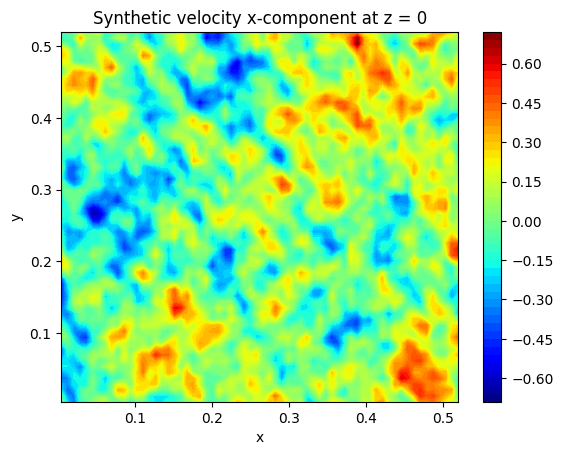
\includegraphics[width=\linewidth]{illustrations/Velocity_Example.png}
    \end{minipage}
    \hfill
    \begin{minipage}{0.49\textwidth}
        \centering
        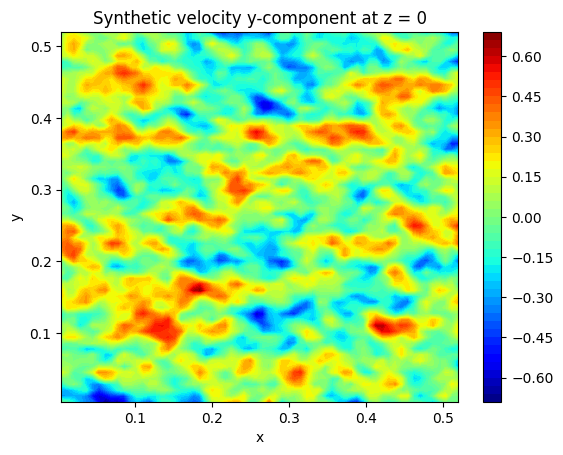
\includegraphics[width=\linewidth]{illustrations/Velocity_Example2.png}
    \end{minipage}
    \caption{Synthetic velocity obtain using the Random Fourier model}
\end{figure}

\begin{figure}[H]
    \centering
    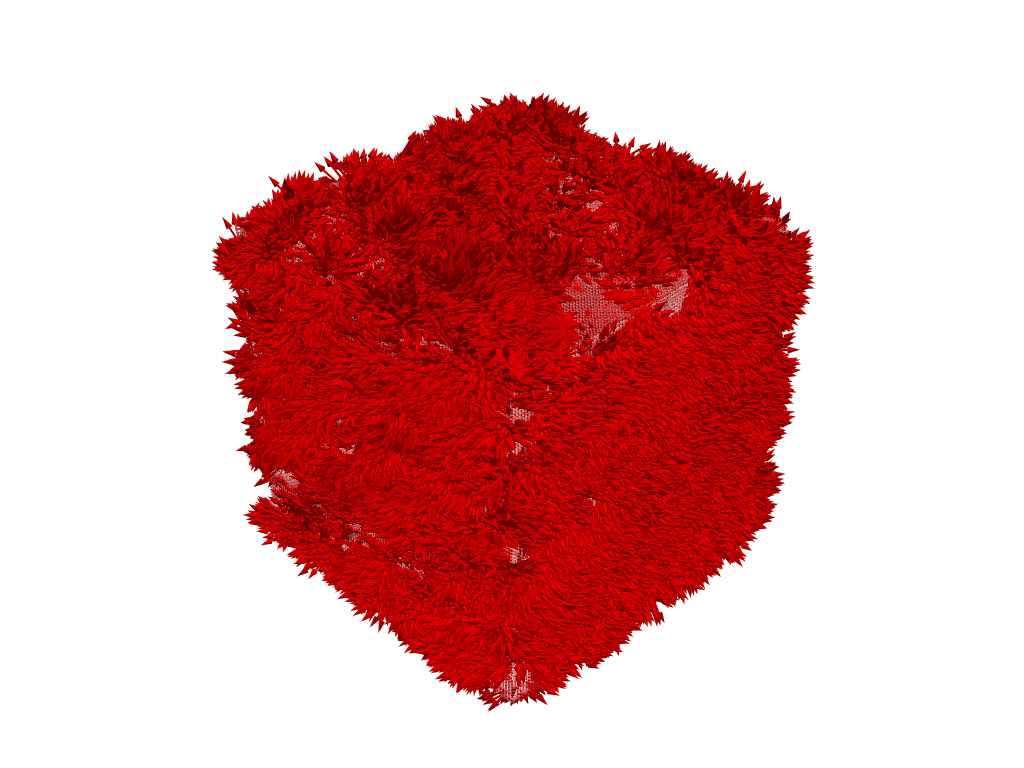
\includegraphics[width=\linewidth]{illustrations/VelocityFieldVTU.png}
    \caption{Synthetic velocity obtain using the Random Fourier model represented by arrows}
\end{figure}

\subsection{Coefficient choice} \label{Coefficient choice}

\begin{figure}[H]
    \centering
    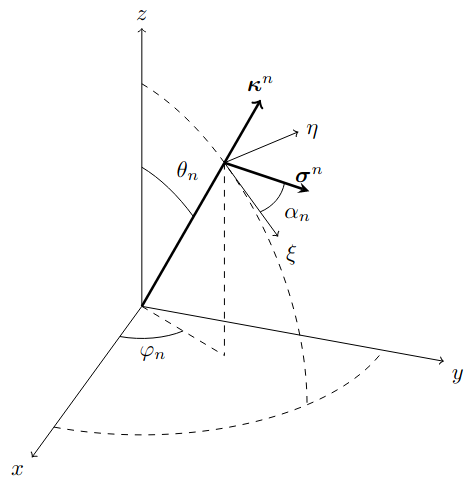
\includegraphics[width=0.5\linewidth]{illustrations/WaveVectorGeometry.png}
    \caption{Wave vector geometry of the $n^\text{th}$ Fourier mode from \cite{Janin2021}}
    \label{WaveVectorGeometry}
\end{figure}
To ensure the statistical isotropy of the generated field, the wave vector $\kappa$ is chosen randomly on the half-sphere.
This leads to the following components choices
\begin{align}
    \kappa_1 &= \sin(\theta)\cos(\varphi) \label{kappa1}\\ 
    \kappa_2 &= \sin(\theta)\sin(\varphi) \label{kappa2}\\
    \kappa_2 & = \cos(\theta) \label{kappa3}
\end{align}
with the angles chosen randomly according to the following probability density functions $f_\theta(x)=\frac{sin(x)}{2}$ and $f_\varphi(x)=\frac{1}{2\pi}\mathbbm{1}_{[0,2\pi]}$. \\
Regarding the choice of $\sigma$, it is such that $\kappa\cdot\sigma=0$ is verified, which is implied by the divergence-free condition $\nabla\cdot u^s=0$. \\
Therefore, 

\begin{align}
    \sigma_1&=\cos(\varphi)\cos(\theta)\cos(\alpha)-\sin(\varphi)\sin(\alpha) \label{sigma1}\\
    \sigma_2&=\sin(\varphi)\cos(\theta)\cos(\alpha)+\cos(\theta)\sin(\alpha) \label{sigma2}\\
    \sigma_3&=-\sin(\theta)\cos(\alpha) \label{sigma3}
\end{align}

with $\alpha$ chosen according to a uniform distribution on $[0,2\pi]$ i.e. $f_\alpha(x)=\frac{1}{2\pi}\mathbbm{1}_{[0,2\pi]}$. \\
The phase coefficient $\psi$ is randomly chosen according to $\mathcal{U}[0,2\pi]$ to ensure spatial homogeneity. \\
Lastly, the amplitude $\hat{u}_n=\sqrt{E(\kappa_n)\delta \kappa_n}$ where $\delta \kappa_n = \frac{\log(\kappa_N)-\log(\kappa_1)}{N}$ and $\kappa_n=e^{(\log(\kappa_1)+n\delta \kappa_n)}$. \\
The method to compute the prescribed energy spectrum $E(\kappa_n)$ is described in the next subsection.

\subsection{Energy spectrum}
Large eddies that carry energy distribute it through the energy cascade to smaller scales until it is dissipated by viscous effect at Kolmogorov scales. 
This energy transfer across different scales is characterized by the energy spectrum, noted $E(\kappa)$. It describes how much kinetic energy is attached to a given wave number $\kappa$. 
\begin{figure}[H]
    \centering
    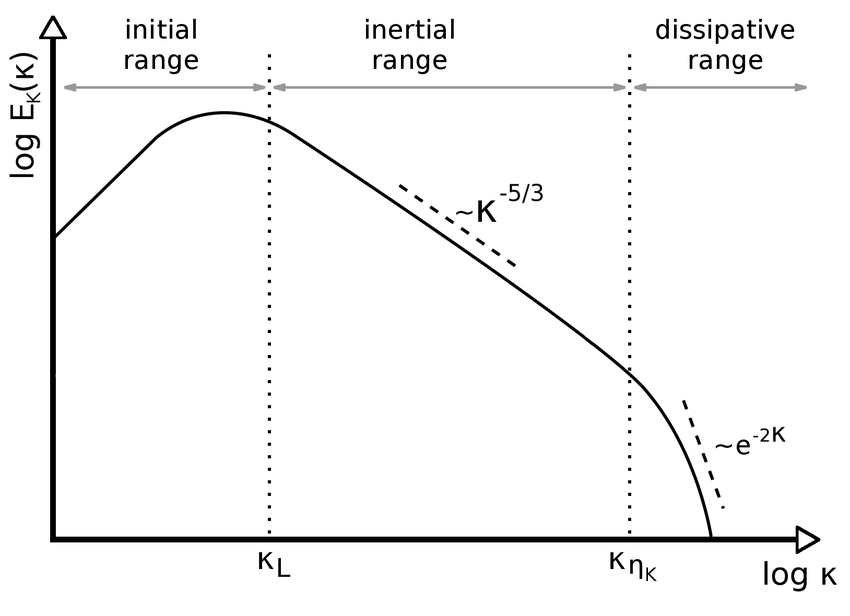
\includegraphics[width=0.7\textwidth]{illustrations/energy-spectrum-example.png}
    \caption{Energy spectrum of a turbulent flow from \cite{phdthesisRies}}
\end{figure}

In the initial range, energy is injected into the flow, for instance, by an obstacle, rotating machinery, or another mechanism. The dynamics in this range are dominated by large eddies. \\
The inertial range is where the energy is transferred without significant dissipation. The large eddies are broken down into smaller eddies and so on.  Finally, in the dissipative range, the viscous effects dominate and the remaining turbulent kinetic energy is dissipated into heat.


\bigskip

In the context of homogeneous isotropic turbulence, Kolmogorov gave the following formula  

\begin{align}
    E(\kappa) = C_k \kappa^{-5/3}\varepsilon^{2/3}
\end{align}
where $\varepsilon$ is the turbulent dissipation, $\kappa$ the wave number and $C_k$ the Kolmogorov constant.

Although this formula captures the behavior in the inertial range and introduces this famous $-\frac{5}{3}$ slop, it fails at reconstructing the spectrum in the initial and dissipative range i.e. at low and high wave numbers. To obtain a more complete recovery of the energy spectrum, \cite{Janin2021} uses, among others, the von-Kármán Pao (VKP) energy spectrum.
\bigskip

It is defined by 

\begin{align}
    E_{\text{VKP}}(\kappa)=\frac{2}{3}\alpha_e k L_e \frac{(kL_e)^4}{[(kL_e)^2+1]^{17/6}}\exp(-2(\kappa L_\eta)^2)
\end{align}

\begin{figure}[H]
    \centering
    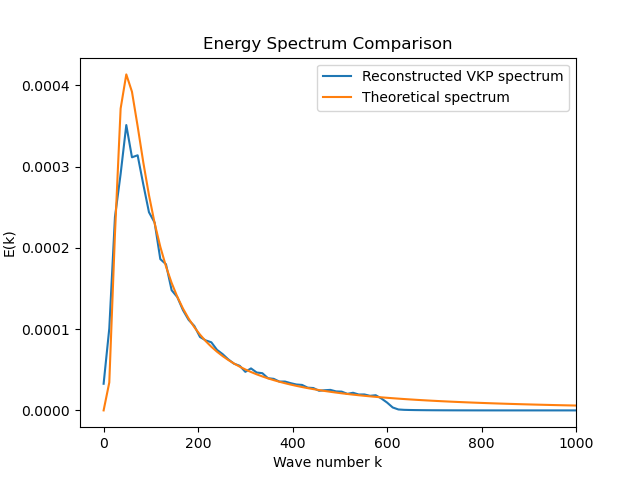
\includegraphics[width=0.7\textwidth]{illustrations/Energy_Spectrum_VKP.png}
    \caption{VKP energy spectrum vs theoretical spectrum}
    \label{VKPspectrum}
\end{figure}

In order to accurately reconstruct the theoretical spectrum, a sufficient number of computational Fourier modes is required. In practice, you don’t include infinitely many modes. We introduce a cutoff wave number which defines the smallest lengths scales that will be resolved. A trade-off naturally arises : if the cutoff is too low, we will miss information the inertial and dissipative range. On the other hand, if the cutoff is too high, we will capture the full inertial range and potentially the Kolmogorov's ones, but it will come at a significant computational cost. Moreover, the smallest scales may not always be physically meaningful, so resolving them is not necessarily worthwhile.

\begin{figure}[H]
    \centering
    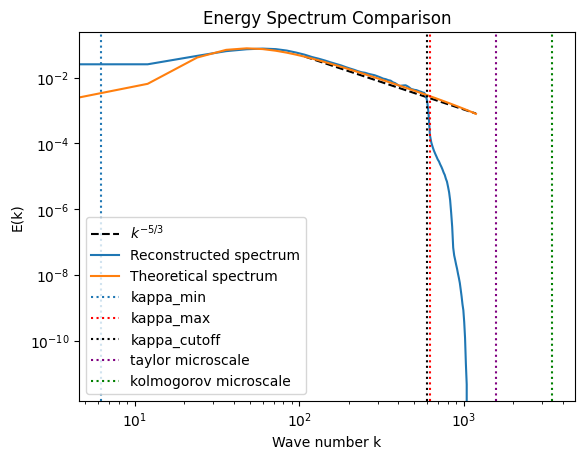
\includegraphics[width=0.7\textwidth]{illustrations/EnergySpectrumTrained.png}
    \caption{VKP energy spectrum vs theoretical spectrum with different scales and the cutoff}
\end{figure}

\begin{comment}
The real energy can be then computed 

\begin{align}
    E = \int_{0}^{\infty}E_{\text{VKP}}(\kappa) d\kappa
\end{align}
\end{comment}

\subsection{Limitations and goals}
The assessment of the synthetic velocity field's quality can be assessed using several metrics. First, the reconstructed energy spectrum should match the thoretical spectrum as closely as possible. Then, for each component, the mean should be zero and the Root Mean Square (RMS) values should match the one used to build the turbulence in the first place. Lastly, the shape of the velocity increments distribution should be examined. \\

\begin{definition}[RMS]
    Let $x=(x_1,\ldots x_n)$ a real vector. The RMS is defined by 
    \begin{align}
        x_\text{RMS} = \sqrt{\frac{1}{n}\sum_{i=1}^{n}x_i^2}
    \end{align}
\end{definition}

\begin{definition}[Velocity increments]
    Let $u$ be a velocity field. For $r>0$ and a point $x$, the velocity increments are defined by 
    \begin{align}
        \delta_r u(x) = u(x+r)-u(x) 
        \label{DefVelIncr}
    \end{align}
\end{definition}

The random Fourier model gives us the following results for each metric.

\begin{table}[h]
\centering
\begin{minipage}{0.45\textwidth}
\centering
\begin{tabular}{ll}
\toprule
\textbf{Direction} & \textbf{Value} \\
\midrule
x & -0.0026918877847492695 \\
y & -0.0001003775978460908 \\
z & -0.0012576839653775096 \\
\bottomrule
\end{tabular}
\caption{Velocity mean}
\label{BaseMean}
\end{minipage}
\hfill
\begin{minipage}{0.45\textwidth}
\centering
\begin{tabular}{ll}
\toprule
\textbf{Direction} & \textbf{Value (expected : 0.222)} \\
\midrule
x & 0.19583044946193695 \\
y & 0.17598901689052582 \\
z & 0.19306901097297668 \\
\bottomrule
\end{tabular}
\caption{RMS speed}
\label{BaseRMSspeed}
\end{minipage}
\end{table}


\begin{figure}[H]
    \centering
    \begin{minipage}{0.49\textwidth}
        \centering
        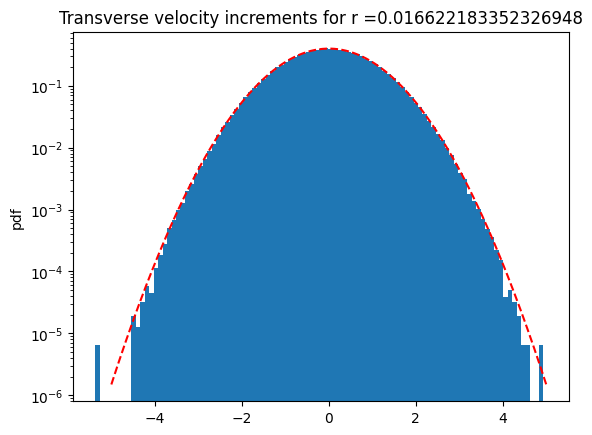
\includegraphics[width=\linewidth]{illustrations/TransVelIncrExample.png}
    \end{minipage}
    \hfill
    \begin{minipage}{0.49\textwidth}
        \centering
        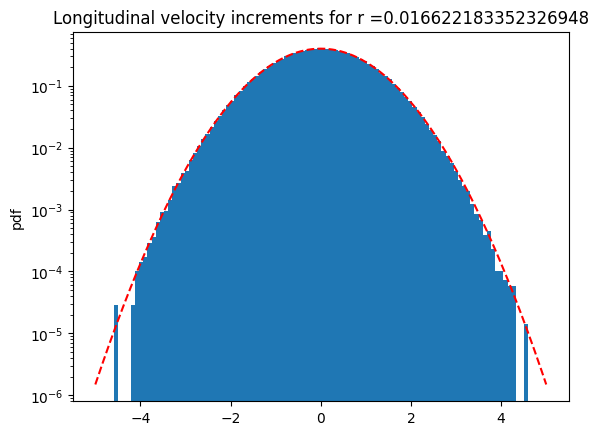
\includegraphics[width=\linewidth]{illustrations/LongVelIncrExample.png}
    \end{minipage}
    \caption{Velocity increments in blue with standard Gaussian in red dots}
\end{figure}


\bigskip
Although, the model retrieve a good energy spectrum (Figure \ref{VKPspectrum}) and limited anisotropy on the RMS speed, the velocity increments obtained are Gaussian. It is known that velocity increments appear to be non-Gaussian and more particularly heavy-tailed distribution. For instance \cite{JIMENEZ1998405} shows that velocity increments display heavy taildness when $r$ is small in \ref{DefVelIncr}.

Furthermore, the following figures show that the more turbulent a flow is, the heavier the tails of its velocity increments are.
\begin{figure}[H]
    \centering
    \begin{minipage}{0.49\textwidth}
        \centering
        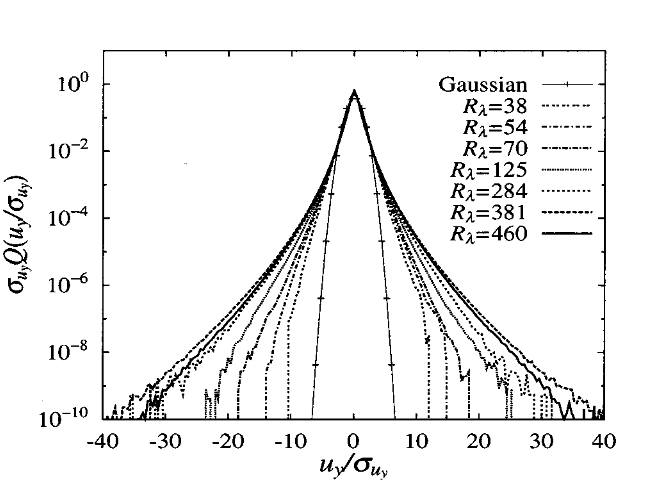
\includegraphics[width=\linewidth]{illustrations/TransVelIncrRe.png}
        \caption{Variation of the transverse velocity derivative PDF with the Reynolds number from \cite{GotohVelIncr}}
    \end{minipage}
    \hfill
    \begin{minipage}{0.49\textwidth}
        \centering
        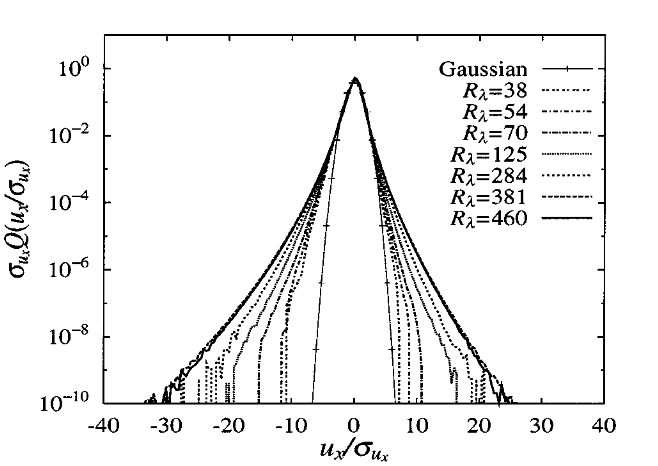
\includegraphics[width=\linewidth]{illustrations/LongVelIncrRe.png}
        \caption{Variation of the longitudinal velocity derivative PDF with the Reynolds number from \cite{GotohVelIncr}}
    \end{minipage}
\end{figure}

\bigskip
With the random Fourier model in mind, the goal is to identify which coefficients could produce more realistic velocity increments without disrupting the other desirable properties that are already satisfied. 

\section{Method} \label{Method}

\subsection{Approach}

Since the goal is to retrieve heavy-tailed velocity increments, the logical criteria to look out is the kurtosis of those increments. 


\begin{definition}[Kurtosis]
    Let $X$ be a real random variable, $\mu$ its mean and $\sigma$ its standard deviation. Its kurtosis is defined by 
    \begin{align}
    \text{kurt}(X)=\mathbb{E}\left[\left(\frac{X-\mu}{\sigma}\right) \right]^2    
    \end{align}
\end{definition}

% \begin{remark}
%     For a Gaussian distribution, which is the distribution of the velocity increments in the first place, the kurtosis is equal to 3.
% \end{remark}

\begin{remark}
    In practice, we look at the kurtosis excess or flatness which is simply $\text{kurt}-3$.
\end{remark}
Therefore, in order to push for heavy tailed velocity increments, we came up with a straight forward flatness loss. 

\begin{definition}[Flatness loss]
    Let $F_\text{target}$ be the target flatness, $x=(x_1,\ldots,x_n)$ be the input vector.
    \begin{align}
        \mathcal{L}_F (x, F_\text{target}) = \frac{1}{N}\sum_{i=1}^{N}\left( \text{kurt}(x)-3 - F_\text{target}  \right) ^2 
    \end{align}
\end{definition}

To compute the energy spectrum as close as the theoretical spectrum, we simply look at the MSE with an added smoothness term. This gave us the following loss

\begin{definition}[Energy spectrum loss]
    Let $\alpha>0$, $E_\text{rec}$ the reconstructed spectrum and $E_\text{theory}$ the theoretical spectrum.
    We define a smoothness term by 
    \begin{align}
        S(E_\text{rec}, E_\text{theory}) = \frac{1}{N-2}\sum_{i=2}^{N-1}\left(E_{\text{rec},i-1} -2E_{\text{rec},i} + E_{\text{rec},i+1}   \right)
    \end{align}
    The loss is then defined by 
    \begin{align}
        \mathcal{L}_{ES}(E_\text{rec}, E_\text{theory}) = \frac{1}{N} \sum_{i=1}^{N} (E_{\text{rec},i}-E_{\text{theory},i})^2 + \alpha S(E_\text{rec}) 
    \end{align} 
\end{definition}

\begin{definition}[Total loss]
    Let $x_L$ be the longitudinal velocity increments, $x_{T}$ the transverse velocity increments and $E_\text{rec}$ the reconstructed energy spectrum.
    \begin{align}
        \mathcal{L} = \mathcal{L}_F(x_L, F_\text{target}) + \mathcal{L}_F(x_T, F_\text{target}) + 1e3 \times\mathcal{L}_{ES}(E_\text{rec}, E_\text{theory})
    \end{align}
    \label{TotalLoss}
\end{definition}



To tackle the problem, several methods were tested, but it turned out simply defining the desired parameter as \texttt{nn.Parameter} in PyTorch and directly optimizing them led to good results. From a computational perspective, this approach was also the most convenient (more on this in \ref{Discussion}). 
\\
In order to optimize the models according to the loss \ref{TotalLoss} we use AdamW and a scheduler. The parameterization of the optimizer was mostly due to empirical evidence (see \ref{OptiParam}).

Although training was typically run for 5000 epochs, convergence was usually achieved after around 2000 epochs. We worked with a target flatness of 15 and $\alpha=0.5$. \\

\subsection{Preliminary work}
In order to check the robustness of the random Fourier model in the first place, we conducted a simple experiment. We set the target flatness as 0, meaning we look for Gaussian velocity increments. Since it is the base model velocity increments, we want to know if we will retrieve the parameterization introduce in \cite{Janin2021} or will it move away. We look up two situations : starting from Gaussian velocity increments and heavy-tailed velocity increments.

\begin{figure}[H]
    \centering
    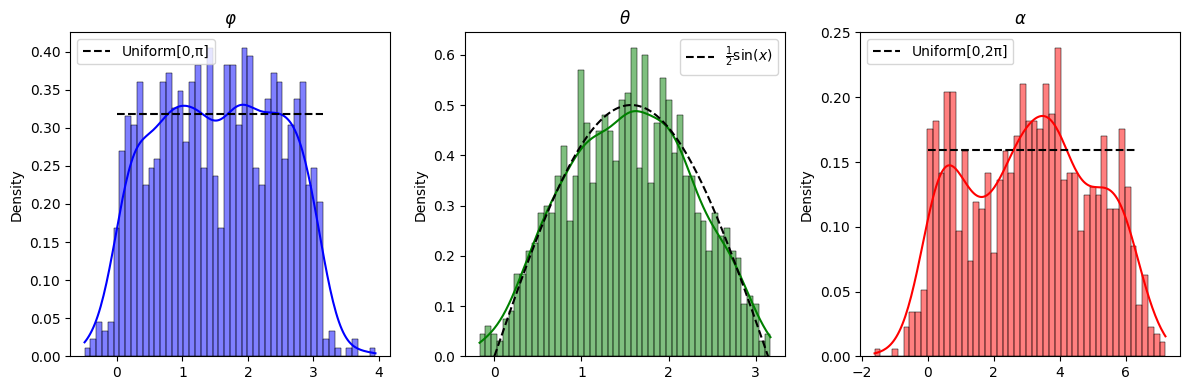
\includegraphics[width=1.0\linewidth]{illustrations/StartGaussian.png}
    \caption{Angles distributions starting from Gaussian velocity increments}
\end{figure}

Here, the angles distributions stay sensibly the same, with a slight change in $\alpha$. This is expected since we already satisfy the target flatness.

\begin{figure}[H]
    \centering
    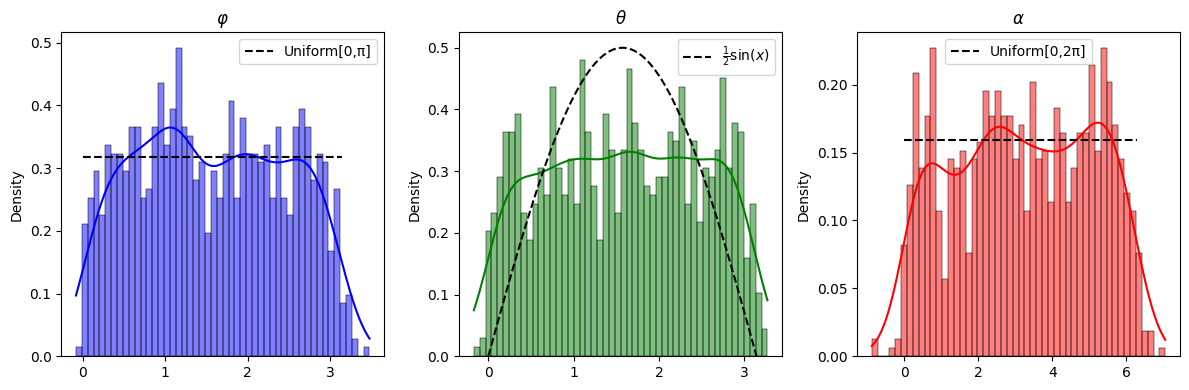
\includegraphics[width=1.0\linewidth]{illustrations/StartHeavyTail.png}
    \caption{Angles distributions starting from heavy-tailed velocity increments}
\end{figure}

In this case, $\varphi$ and $\alpha$ stay relatively stable but $\theta$ is drawn to a more spread distribution. 

\bigskip
In both cases Gaussian velocity increments are indeed recovered, the RMS speed are in the same range as in \ref{BaseRMSspeed} and the generated velocity field does average to 0.

\subsection{Phase coefficient}
To improve the situation, our first idea was to work on the phase parameter $\psi$ in \ref{RandomFourierModel}, with the idea of finding a better distribution than $\mathcal{U}([0,2\pi])$. A simple experiment consisting of changing $\mathcal{U}[0,2\pi]$ to arbitrary distribution like $\mathcal{N}(-10,130)$ or $\mathcal{E}(1)$ showed that it has no effect on the shape of the velocity increments distribution. Indeed, the reason is pretty straight forward : the Central Limit Theorem (CLT). \\
Sampling I.I.D. values of $\psi$ according to any of these distributions and plugging it in $\ref{RandomFourierModel}$ with sufficiently large $N$ (which is expected in our situation) leads directly to the conditions of the CLT.

\bigskip
Applying the approach described in  \ref{Method} didn't produce satisfying results and focusing solely on $\psi$ was ultimately abandoned.



\subsection{Phase, wave vector and direction}
The natural follow-up was to look at all the coefficient all together, i.e. $(\psi,\kappa,\sigma)$, without changing the objectives nor the method. It led to heavy tailed velocity increments indeed as shown in figure \ref{fig:VelIncrPSIKAPPASIGMA}.

\begin{figure}[H]
    \centering
    \begin{minipage}{0.48\textwidth}
        \centering
        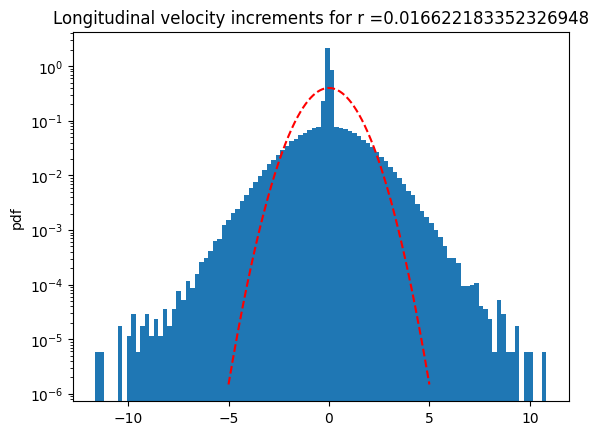
\includegraphics[width=\linewidth]{VelIncrPSIKAPPASIGMA/VelIncrLong.png}
    \end{minipage}\hfill
    \begin{minipage}{0.48\textwidth}
        \centering
        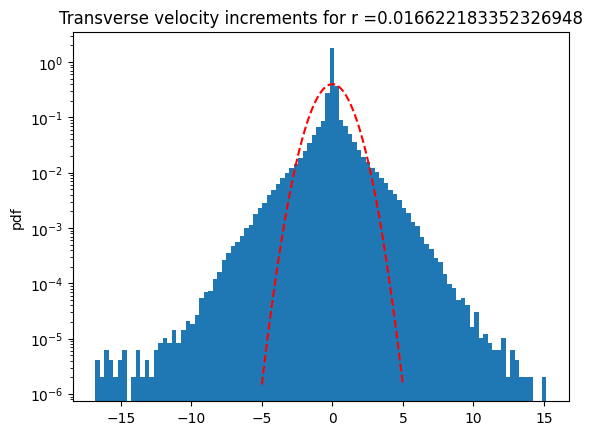
\includegraphics[width=\linewidth]{VelIncrPSIKAPPASIGMA/VelIncrTrans.png}
    \end{minipage}
    \caption{Velocity increments with learned coefficient \((\psi,\kappa,\sigma)\) and standard Gaussian in red dots}
    \label{fig:VelIncrPSIKAPPASIGMA}
\end{figure}

The reconstructed spectrum shows a considerable bias and doesn't capture the small scales correctly.

\begin{figure}[H]
    \centering
    \begin{minipage}{0.49\textwidth}
        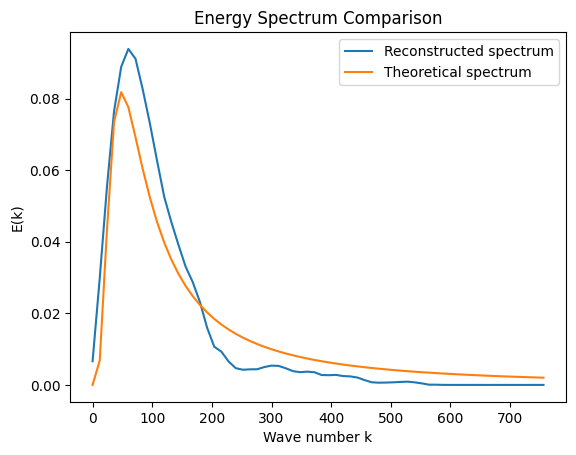
\includegraphics[width=\linewidth]{VelIncrPSIKAPPASIGMA/EnergySpectrum.png}
        \caption{Energy spectrum with the learned parameters $(\psi,\kappa,\sigma)$}
        \label{fig:EnergySpectrumPsiKappaSigma}
    \end{minipage} \hfill
        \begin{minipage}{0.49\textwidth}
        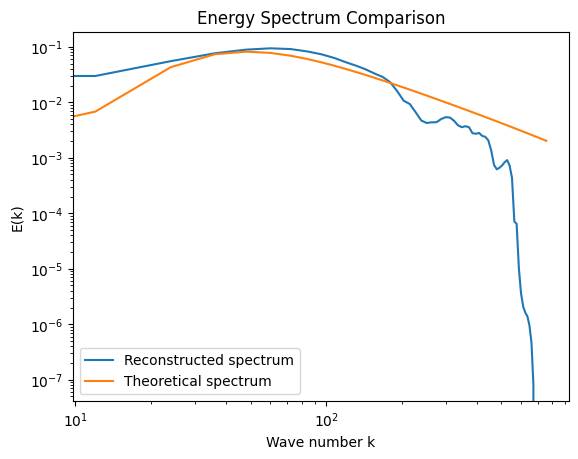
\includegraphics[width=\linewidth]{VelIncrPSIKAPPASIGMA/EnergySpectrumLog.png}
        \caption{Energy spectrum with the learned parameters $(\psi,\kappa,\sigma)$ with log scale}
        \label{fig:EnergySpectrumLogPsiKappaSigma}
    \end{minipage}
    \end{figure}

\begin{table}[h]
\centering
\begin{minipage}{0.45\textwidth}
\centering
\begin{tabular}{ll}
\toprule
\textbf{Direction} & \textbf{Value} \\
\midrule
x & 7.787999493302777e-05 \\
y & 5.701697227777913e-05 \\
z & -0.030603401362895966 \\
\bottomrule
\end{tabular}
\caption{Velocity mean}
\label{PsiKappaSigmaMean}
\end{minipage}
\hfill
\begin{minipage}{0.45\textwidth}
\centering
\begin{tabular}{ll}
\toprule
\textbf{Direction} & \textbf{Value (expected : 0.222)} \\
\midrule
x & 0.0017423529643565416 \\
y & 0.0006628130213357508 \\
z & 0.889664888381958 \\
\bottomrule
\end{tabular}
\caption{RMS speed}
\label{PsiKappaSigmaRMS}
\end{minipage}
\end{table}

\begin{comment}
On the learned parameters, we fit a Gaussian kernel density estimator and obtain the marginal distribution

\begin{figure}[H]
    \centering
    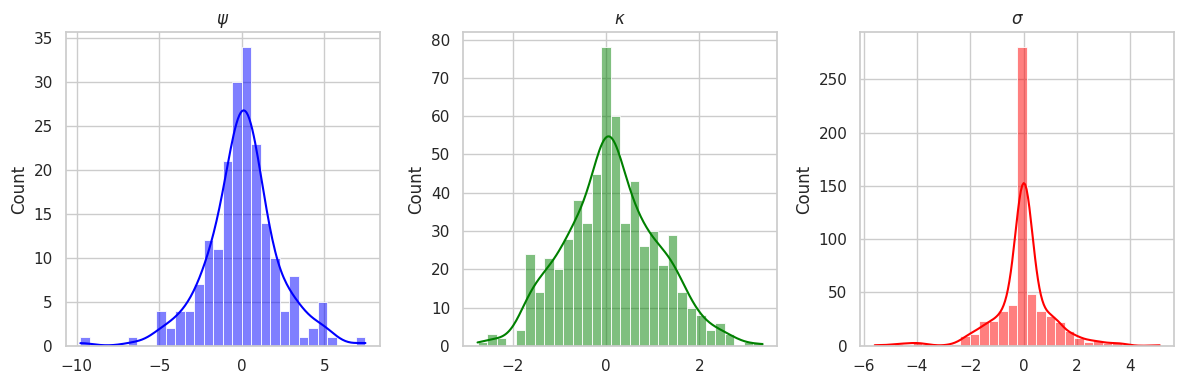
\includegraphics[width=\linewidth]{VelIncrPSIKAPPASIGMA/Distributions.png}
    \label{fig:Distributions3}
    \caption{Marginal density of the learned parameters $(\psi,\kappa,\sigma)$}
    \label{MarginalsPsiKappaSigma}
\end{figure}

What we found is to generate new triplet $(\psi,\kappa,\sigma)$ sampling directly according to the marginal distributions from \ref{MarginalsPsiKappaSigma} doesn't work but sampling according to the obtained joint distribution led to a mild flatness of the velocity increments.

\begin{figure}[H]
    \centering
    \begin{minipage}{0.49\textwidth}
        \centering
        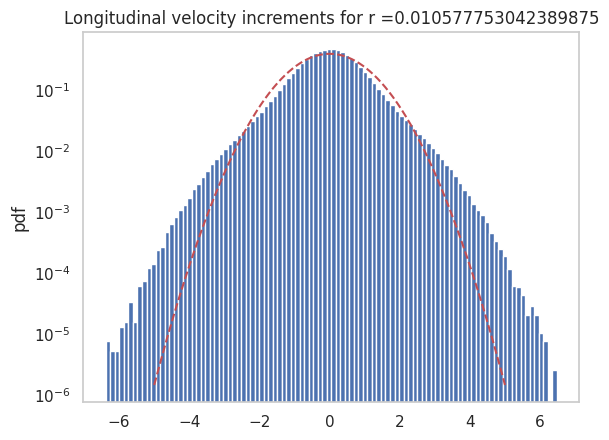
\includegraphics[width=\linewidth]{VelIncrPSIKAPPASIGMA/GenIncrLong.png}
        \label{fig:GenIncrLong3}
    \end{minipage}\hfill
    \begin{minipage}{0.49\textwidth}
        \centering
        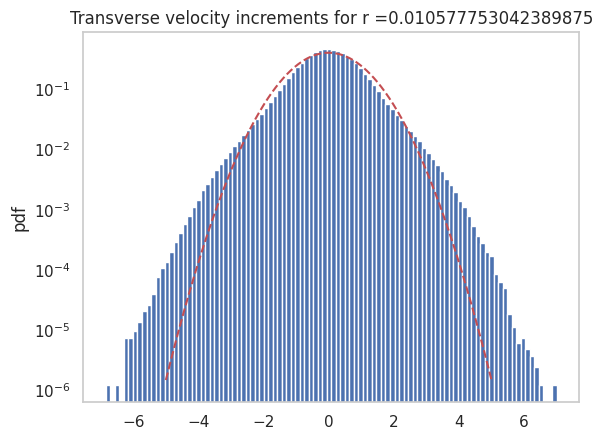
\includegraphics[width=\linewidth]{VelIncrPSIKAPPASIGMA/GenIncrTrans.png}
        \label{fig:GenIncrTrans3}
    \end{minipage}
    \caption{Velocity increments with sampled coefficient \((\psi,\kappa,\sigma)\) and standard Gaussian in red dots}
\end{figure}
\end{comment}

Although, this approach works as it produces heavy tailed velocity increments, it exhibits serious anisotropy and fails to recover a good energy spectrum.\\
Furthermore, there is no guarantee that the obtained $\kappa$ and $\sigma$ are orthogonal to each other as stated in \ref{Coefficient choice}. \\
Therefore, we shift our focus on the angles $(\varphi,\theta,\alpha)$ composing the $\kappa$ and $\sigma$ component. We aim at learning the three angles while using \ref{kappa1}, \ref{kappa2},\ref{kappa3} and \ref{sigma1},\ref{sigma2},\ref{sigma3} to preserve the identity $\kappa\cdot\sigma=0$.


\subsection{Angles}
Since we want to work on the angles, we need to make sure the angles are always coherent with the geometry (see \ref{WaveVectorGeometry}). Therefore, to make sure that $\varphi, \theta$ and $\alpha$ lives in their respective domain $[0,\pi], [0,\pi]$ and $[0,2\pi]$.

We train the model on 500 modes with $100^3$ points, with the turbulence parameter described in \ref{TurbulenceParameters} and retrieve great velocities increments.

\begin{figure}[H]
    \centering
    \begin{minipage}{0.49\textwidth}
        \centering
        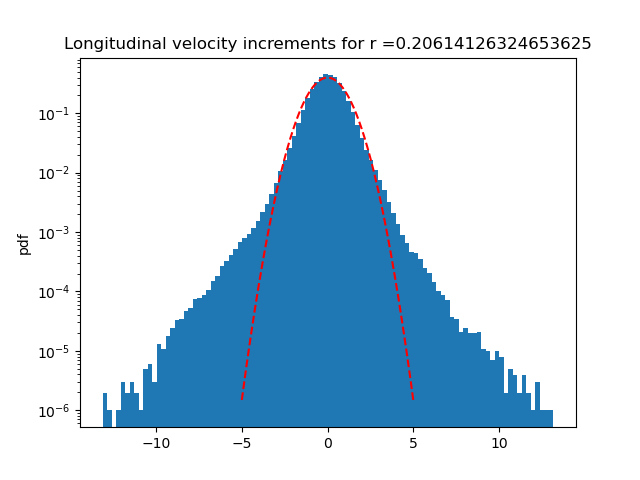
\includegraphics[width=\linewidth]{illustrations/LongVelIncrAngles.png}
        \label{fig:VelIncrLongAngles}
    \end{minipage}\hfill
    \begin{minipage}{0.49\textwidth}
        \centering
        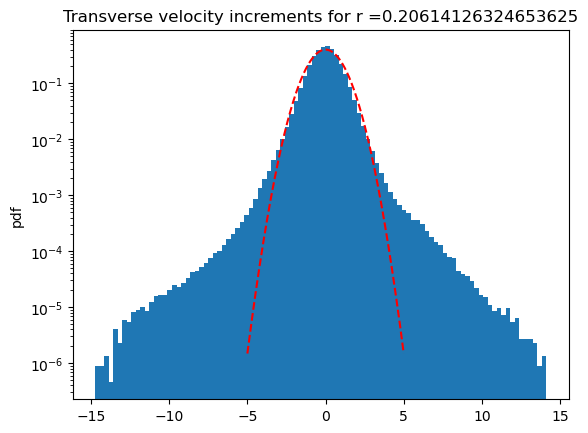
\includegraphics[width=\linewidth]{illustrations/TransVelIncrAngles.png}
        \label{fig:VelIncrTransAngles}
    \end{minipage}
    \caption{Velocity increments with learned angles \((\varphi,\theta,\alpha)\) and standard Gaussian in red dots}
\end{figure}

Unlike in \ref{fig:EnergySpectrumLogPsiKappaSigma}, here the energy spectrum is accurately reconstructed but nowhere near the one from \ref{PsiKappaSigmaRMS}.

\begin{figure}[H]
    \centering
    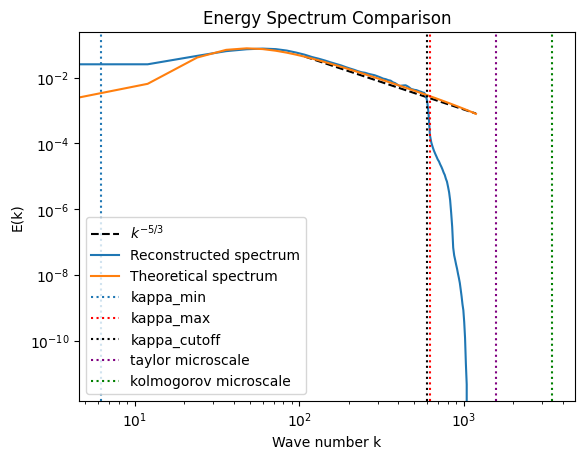
\includegraphics[width=0.7\linewidth]{illustrations/EnergySpectrumTrained.png}
    \caption{Energy spectrum reconstructed after training}
    \label{EnergySpectrumAngles}
\end{figure}

However, a slight anisotropy is displayed in the RMS speed obtained.
\begin{table}[h]
\centering
\begin{minipage}{0.45\textwidth}
\centering
\begin{tabular}{ll}
\toprule
\textbf{Direction} & \textbf{Value} \\
\midrule
x & 0.0025640586391091347 \\
y & -0.00652820710092783 \\
z & -0.0009377452079206705 \\
\bottomrule
\end{tabular}
\caption{Velocity mean}
\label{AnglesMean}
\end{minipage}
\hfill
\begin{minipage}{0.45\textwidth}
\centering
\begin{tabular}{ll}
\toprule
\textbf{Direction} & \textbf{Value (expected : 0.222)} \\
\midrule
x & 0.12904468178749084 \\
y & 0.3165183663368225 \\
z & 0.11406964063644409 \\
\bottomrule
\end{tabular}
\caption{RMS speed}
\label{AnglesRMS}
\end{minipage}
\end{table}

We obtain the following marginal distribution.
\begin{figure}[H]
    \centering 
    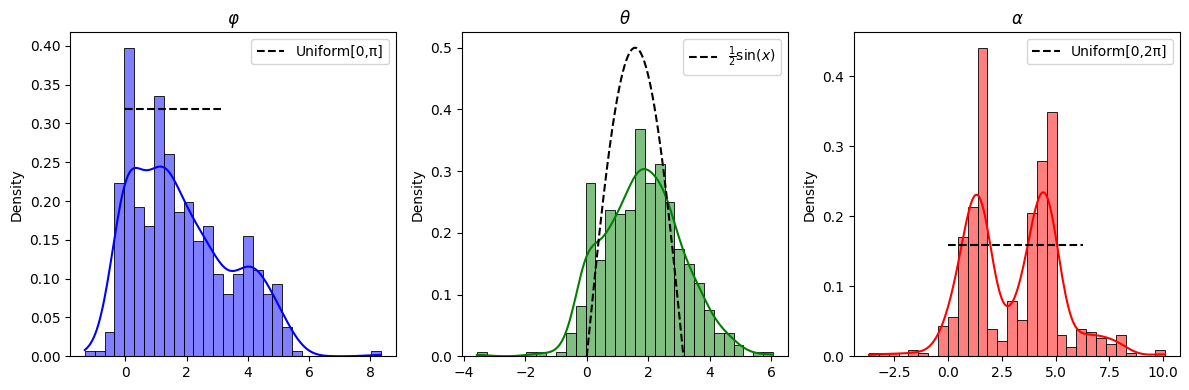
\includegraphics[width=1.0\linewidth]{illustrations/AnglesDistributionLearned.png}
    \caption{Marginal distribution of the learned angles with the base distribution in black dots}
\end{figure}

\subsubsection{Robustness}
Additionally, these angles exhibit strong robustness to changes in the turbulence characteristics. When the kinetic energy is doubled (by multiplying the RMS speed in \ref{TurbulenceParameters} by $\sqrt{2}$), the length of the periodic box is doubled, or both are changed simultaneously, the quality of the velocity increments remains consistent. The resulting anisotropy and energy spectrum remain as accurate as those shown in \ref{AnglesRMS} and \ref{EnergySpectrumAngles}.

\section{Discussion} \label{Discussion}
% Overall, retrieving non-Gaussian velocity increments leads RMS speed that are off. 
% The work was highly exploratory and featured trials and errors along the way. 

Different architectures were explored to address the problem and also bring new generalization possibilities, such as generating new instances of angles for a specific turbulent case. Unfortunately, significant computational challenges were encountered. \\
At the time of writing, I got my hands on an Nvidia A10 GPU which I am working with to try more complex solution that won't be featured in this work. \\
In reality, the complexity and the computational bottleneck arises mainly with the number of points considered. A low-resolution grid leads to under-resolved fields, which directly impacts the accuracy of velocity increments computed via the discretization in \ref{DefVelIncr}. \\
The code used to generate all results presented in this work will be made available at: \href{https://github.com/SamyBraik/InternshipCode}{GitHub repository}
\newpage

\section{Conclusion}
In this work, we focused on improving the generation of synthetic turbulent velocity fields using the random Fourier model, with the specific goal of producing velocity increments exhibiting heavy-tailed statistics, as observed in real turbulence. We reviewed the limitations of the standard random Fourier approach, which, while accurately reconstructing the energy spectrum and maintaining near-zero mean velocities, produces Gaussian velocity increments that fail to capture the intermittency characteristic of turbulence.

\bigskip
Our approach centered on directly optimizing the coefficients of the Fourier modes, and more specifically the angles defining the wave vectors and directions, to control the statistical properties of the velocity increments. By introducing a flatness-based loss in combination with an energy spectrum loss, we were able to generate heavy-tailed velocity increments while preserving the overall energy distribution. The learned angle distributions proved robust to changes in turbulence parameters and maintained reasonable isotropy, demonstrating the generality of the approach.

\bigskip
While optimizing the full set of coefficients 
$(\psi,\kappa,\sigma)$
 produced heavy tails, it led to strong anisotropy and a biased energy spectrum. Focusing on the angle parameterization allowed us to overcome these limitations, balancing the statistical accuracy of velocity increments with the physical consistency of the field.

 \bigskip
Overall, our work highlights the potential of targeted parameter optimization in synthetic turbulence generation, providing a method for producing velocity fields that better reflect the non-Gaussian features of real turbulence. Future work could extend this approach to unfrozen turbulence, incorporating temporal effects and ultimately quit the HIT framework to look at anisotropic turbulence to get closer to realistic scenarios. 


% \begin{comment}
\newpage
\appendix

\section{Turbulence parameters}
To generate the turbulence several physical and spectral parameters have to be given as input for the model. Throughout the report the parameters that have been used are listed in the following table. 

\begin{center}
\begin{tabular}{lll}
\toprule
\textbf{Parameter} & \textbf{Value} & \textbf{Unit}\\
\midrule
Number of points             & $64^3$ or $100^3$ & -- \\
Length of the periodic box   & $\tfrac{\pi}{6}$ & \si{\meter}\\
Number of modes              & 250 or 500 & --\\
RMS speed                    & 0.222 & \si{\meter\per\second}\\
Integral length scale        & 0.024 & \si{\meter} \\
Kinetic energy               & $1.5 \times (0.222^2)$ & \si{\meter\squared\per\second\squared} \\
Viscosity                    & $1.8 \times 10^{-5}$ & \si{\meter\squared\per\second} \\
Minimum wave number          & $\tfrac{2\pi}{1.0}$ & \si{\per\meter}\\
Maximum wave number          & $\tfrac{2\pi}{0.01}$ & \si{\per\meter}\\
\bottomrule
\end{tabular}
\label{TurbulenceParameters}
\end{center}

\section{Optimizer hyperparameters} \label{OptiParam}
% \begin{comment}
\begin{minted}{python}
optimizer = torch.optim.AdamW(
    model.parameters(),
    lr=1e-3,          
    weight_decay=1e-4
)

scheduler = torch.optim.lr_scheduler.ReduceLROnPlateau(
    optimizer,
    mode='min',       
    factor=0.5,       
    patience=50,      
    threshold=1e-3,   
    min_lr=1e-6,      
    cooldown=10       
)
\end{minted}
% \end{comment}

\section{Variable selection}
To address the question of which angles are the most influential and which one could be negligible, we simply perform a case analysis. In the same training context, we varied individual angles while keeping others froze and untrained. It gave us the following results.

\begin{table}[!htb]
    \caption{Losses obtain for different parameter combination}
    \begin{subtable}{.5\linewidth}
      \centering
        \caption{250 modes}
        \begin{tabular}{ c | c | c }
        Parameters & Loss & RMS (x, y, z)\\
        \hline
        $(0,0,\alpha)$ & 123.24456 & (0.24, 0.08, 0.12)\\
        $(0, \theta, 0)$ & 1.50244 & (0.22, 0.11, 0.08)\\
        $(0, \theta,\alpha)$ & 65.67394 & (0.11, 0.22, 0.09)\\
        $(\varphi, 0, 0)$ & 0.75362 & (0.09, 0.24, 0.06)\\
        $(\varphi, 0, \alpha)$ & 0.74764 & (0.20, 0.10, 0.09)\\
        $(\varphi,\theta, 0)$ & 0.75258 & (0.12, 0.22, 0.04)\\
        $(\varphi,\theta,\alpha)$ & 2.15906 & (0.22, 0.11, 0.09)\\
    \end{tabular}
    \end{subtable}%
    \begin{subtable}{.5\linewidth}
      \centering
        \caption{500 modes}
        \begin{tabular}{ c | c | c }
        Parameters & Loss & RMS (x, y, z)\\
        \hline
        $(0,0,\alpha)$ & 0.73864 & (0.14, 0.20, 0.06)\\
        $(0, \theta, 0)$ & 0.74741 & (0.20, 0.11, 0.10)\\
        $(0, \theta,\alpha)$ & 0.79737 & (0.14, 0.21, 0.09)\\
        $(\varphi, 0, 0)$ & 0.75514 & (0.10, 0.22, 0.08)\\
        $(\varphi, 0, \alpha)$ & 0.74716 & (0.21, 0.11, 0.09)\\
        $(\varphi,\theta, 0)$ & 0.74118 & (0.22, 0.09, 0.11)\\
        $(\varphi,\theta,\alpha)$ & 0.75355 & (0.20, 0.13, 0.09)\\
        \end{tabular}
    \end{subtable} 
\end{table}


Overall, the more modes the better it is. A lot of the cases are pretty close together and lead to sensibly the same losses and in practice the desired flatness and a good recovery of the energy spectrum. \\
RMS values are affected after the learning step, depending on which angles are considered. For the moment, adding a loss on those RMS values tend to lead to less flat tails on the output velocities increments. A trade-off between RMS and flat tails seems to arise. For instance, in the case where all the parameters are learned, like in the previous section, the RMS for the z direction is off (0.09 with an expected value of 0.222).

%It appears that considering all three parameters gives the best result, which makes sense since it allow more degrees of freedom. It also highlight the importance of \(\alpha\). If we constaint the model to two parameters (or even one), including alpha consistently leads to better results. Moreover, \(\theta\) is second on the list. Constraining the number of parameters to two, the case \((\theta,\alpha)\) is preferred to the case \((\varphi,\alpha)\).

\subsection{Marginal distributions}
\begin{figure}[H]
    \centering
    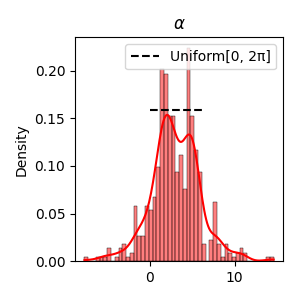
\includegraphics[height=0.35\textwidth]{VariableSelection/alpha.png}
    \label{fig:Distributions4.1}
    \caption{Marginal density of the learned parameters \((\alpha)\)}
\end{figure}
\begin{figure}[H]
    \centering
    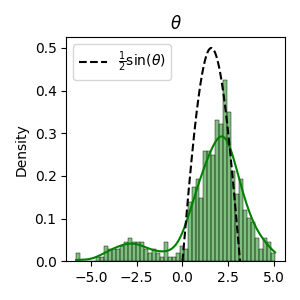
\includegraphics[height=0.35\textwidth]{VariableSelection/theta.png}
    \label{fig:Distributions4.2}
    \caption{Marginal density of the learned parameters \((\theta)\)}
\end{figure}
\begin{figure}[H]
    \centering
    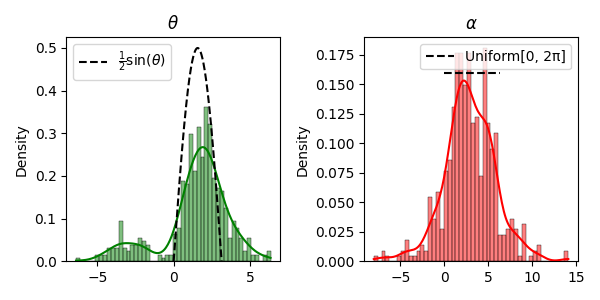
\includegraphics[height=0.35\textwidth]{VariableSelection/theta_alpha.png}
    \label{fig:Distributions4.3}
    \caption{Marginal density of the learned parameters \((\theta,\alpha)\)}
\end{figure}
\begin{figure}[H]
    \centering
    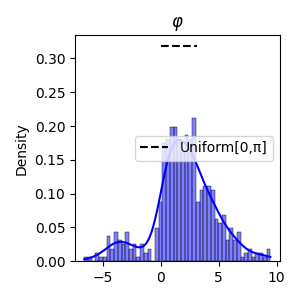
\includegraphics[height=0.35\textwidth]{VariableSelection/phi.png}
    \label{fig:Distributions4.4}
    \caption{Marginal density of the learned parameters \((\varphi)\)}
\end{figure}
\begin{figure}[H]
    \centering
    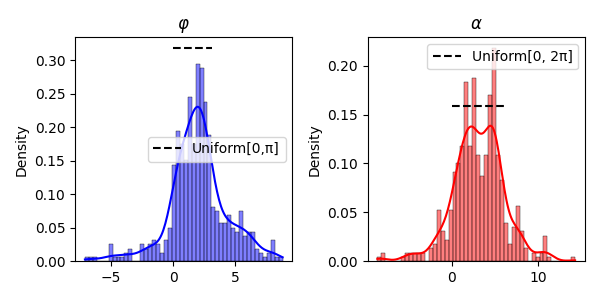
\includegraphics[height=0.35\textwidth]{VariableSelection/phi_alpha.png}
    \label{fig:Distributions4.5}
    \caption{Marginal density of the learned parameters \((\varphi,\alpha)\)}
\end{figure}
\begin{figure}[H]
    \centering
    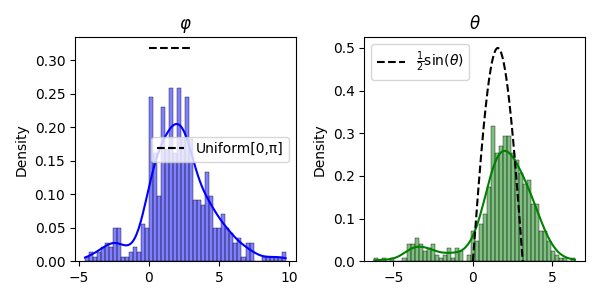
\includegraphics[height=0.35\textwidth]{VariableSelection/phi_theta.png}
    \label{fig:Distributions4.6}
    \caption{Marginal density of the learned parameters \((\varphi,\theta)\)}
\end{figure}
\begin{figure}[H]
    \centering
    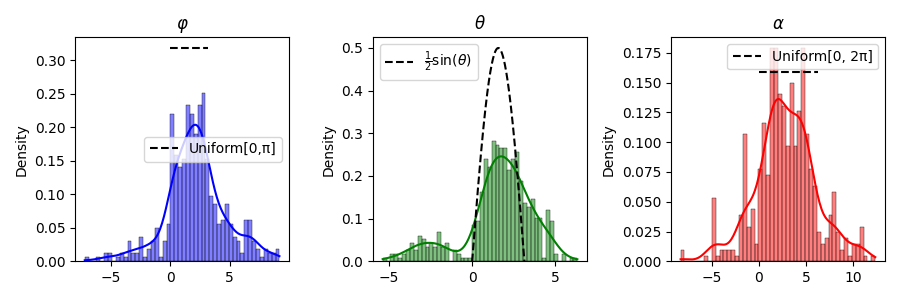
\includegraphics[height=0.35\textwidth]{VariableSelection/phi_theta_alpha.png}
    \label{fig:Distributions4.7}
    \caption{Marginal density of the learned parameters \((\varphi,\theta,\alpha)\)}
\end{figure}

We can see that among all the cases, the final marginal distributions seem pretty consistent throughout.


\subsection{Joint distributions}

\begin{figure}[H]
    \centering

    \begin{subfigure}[b]{0.45\textwidth}
        \centering
        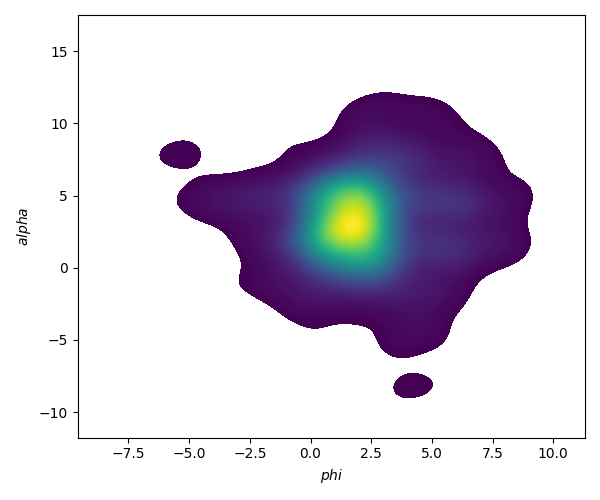
\includegraphics[width=\textwidth]{VariableSelection/joint_phi_alpha.png}
        \caption{Learned parameters \((\varphi, \alpha)\)}
        \label{fig:joint_phi_alpha}
    \end{subfigure}
    \hfill
    \begin{subfigure}[b]{0.45\textwidth}
        \centering
        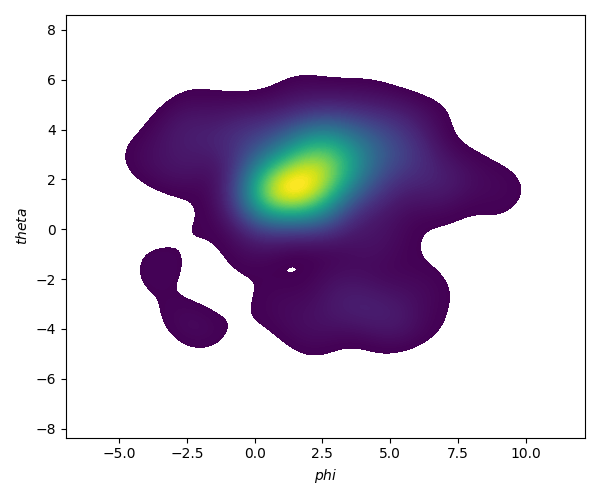
\includegraphics[width=\textwidth]{VariableSelection/joint_phi_theta.png}
        \caption{Joint distribution of \((\varphi, \theta)\)}
        \label{fig:joint_phi_theta}
    \end{subfigure}

    \vspace{0.5em}

    \begin{subfigure}[b]{0.45\textwidth}
        \centering
        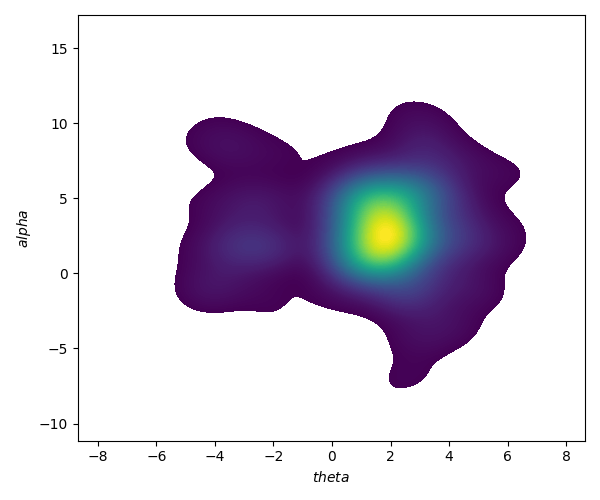
\includegraphics[width=\textwidth]{VariableSelection/joint_theta_alpha.png}
        \caption{Joint distribution of \((\theta, \alpha)\)}
        \label{fig:joint_theta_alpha}
    \end{subfigure}
    \hfill
    \begin{subfigure}[b]{0.45\textwidth}
        \centering
        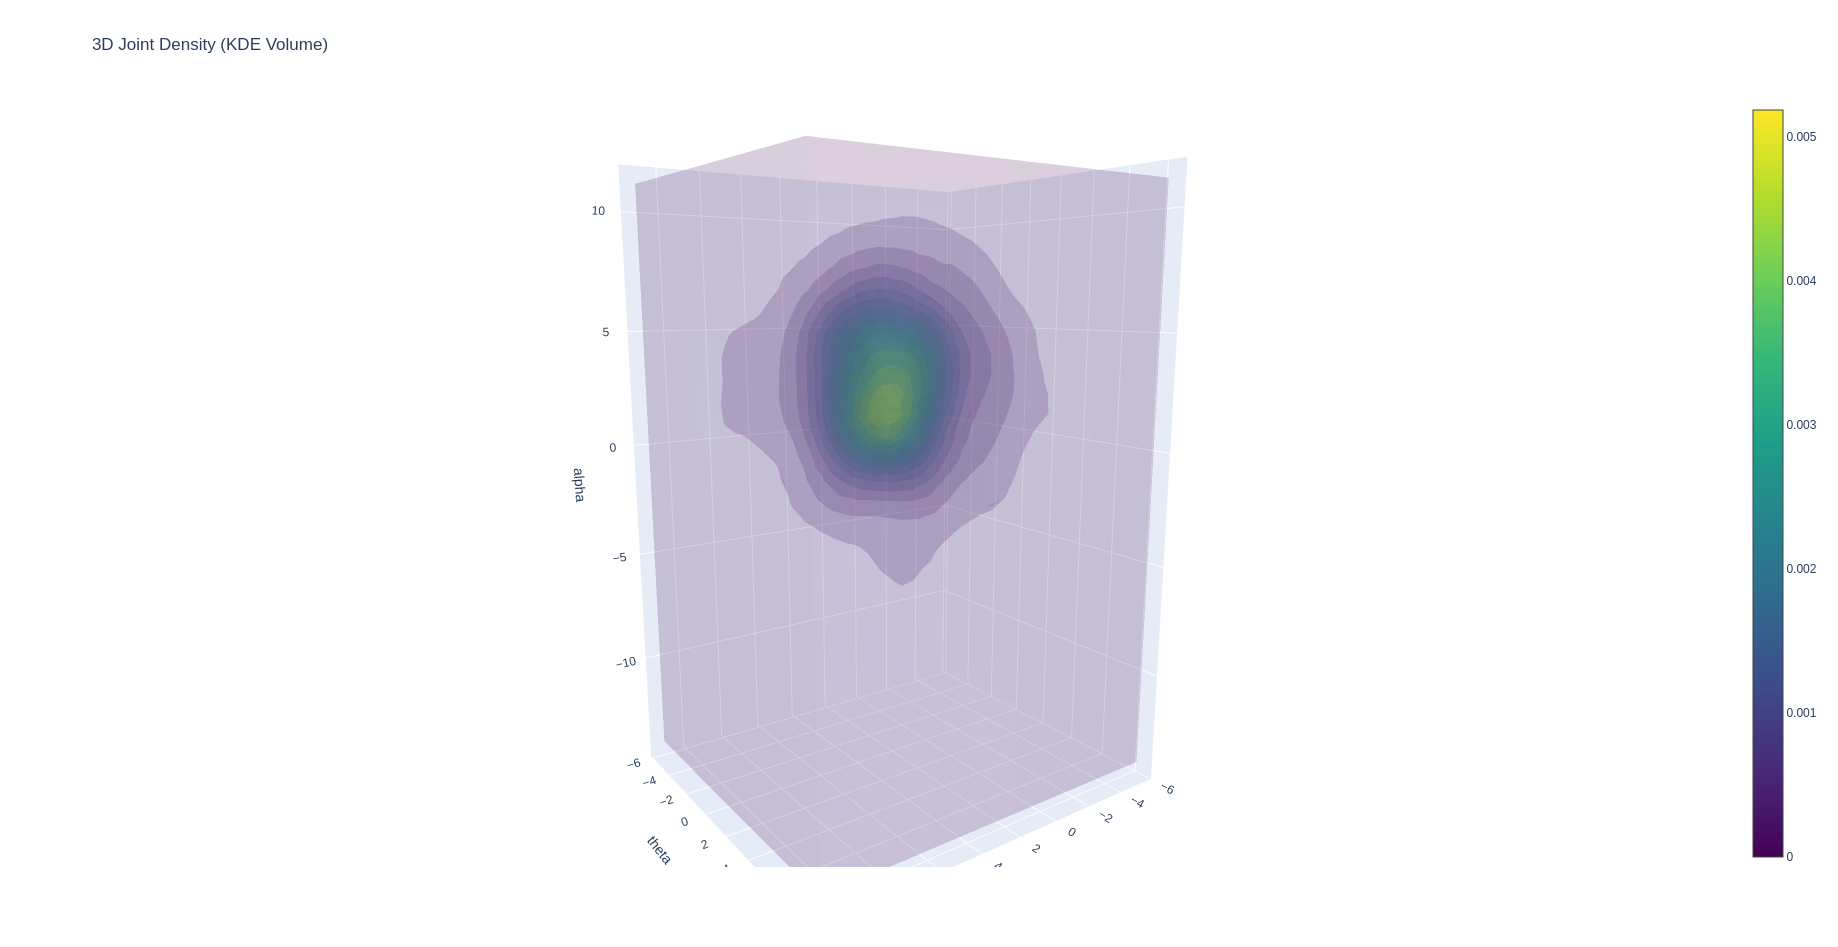
\includegraphics[width=\textwidth]{VariableSelection/joint3D.png}
        \caption{Joint distribution of \((\varphi, \theta, \alpha)\)}
        \label{fig:joint3D}
    \end{subfigure}

    \caption{Joint distributions of parameter combination}
    \label{fig:joint_distributions}
\end{figure}

\section{Variable selection with \(\psi\)}
We repeat the previous experiment considering also the phase coefficient \(\psi\). 

\bigskip
%When introducing \(\psi\), the earlier conclusion that \(\alpha\) is the most important coefficient appear to no longer hold. The three cases with the lowest loss are, in fact, those where \(\alpha\) is excluded. 

%Same observation as before could be made, the greater the loss with 250 modes, the smaller it is with 500 modes.


\begin{table}[!htb]
    \caption{Losses obtain for different parameter combination}
    \begin{subtable}{.5\linewidth}
      \centering
        \caption{250 modes}
        \begin{tabular}{ c | c | c}
        Parameters & Loss & RMS (x, y, z)\\
        \hline
        $(0,0,\alpha,\psi)$ & 0.75522 & (0.20, 0.11, 0.10)\\
        $(\varphi,0, \alpha,\psi)$ & 0.74388 & (0.09, 0.22, 0.04)\\
        $(\varphi, 0,0,\psi)$ & 0.73930 & (0.11, 0.22, 0.08)\\
        $(0, \theta, 0,\psi)$ & 24.56362 & (0.12, 0.22, 0.06)\\
        $(0,\theta, \alpha,\psi)$ & 0.75160 & (0.21, 0.12, 0.10)\\
        $(\varphi,\theta,0,\psi)$ & 0.81957 & (0.09, 0.21, 0.08)\\
        $(\varphi,\theta,\alpha,\psi)$ & 183.87051 & (0.11, 0.27, 0.05)\\
        \end{tabular}
    \end{subtable}%
    \begin{subtable}{.5\linewidth}
      \centering
        \caption{500 modes}
        \begin{tabular}{ c | c | c}
        Parameters & Loss & RMS (x, y, z)\\
        \hline
        $(0,0,\alpha,\psi)$ & 0.74805 & (0.11, 0.25, 0.07)\\
        $(\varphi,0, \alpha,\psi)$ & 0.74443 & (0.21, 0.17, 0.06)\\
        $(\varphi, 0,0,\psi)$ & 0.74356 & (0.09, 0.27, 0.06)\\
        $(0, \theta, 0,\psi)$ & 0.74534 & (0.20, 0.11, 0.10)\\
        $(0,\theta, \alpha,\psi)$ & 0.74584 & (0.20, 0.14, 0.10)\\
        $(\varphi,\theta,0,\psi)$ & 0.73757 & (0.20, 0.12, 0.11)\\
        $(\varphi,\theta,\alpha,\psi)$ &  3.38473  & (0.23, 0.11, 0.09)\\
        \end{tabular}
    \end{subtable}
\end{table}

\subsection{Marginal distributions}

\begin{figure}[H]
    \centering
    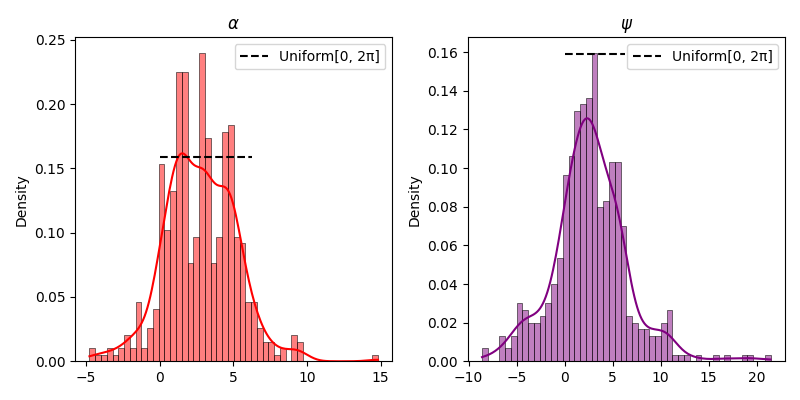
\includegraphics[height=0.35\textwidth]{VariableSelectionPsi/alpha_psi.png}
    \caption{Marginal density of the learned parameters \((\alpha,\psi)\)}
    \label{fig:Distributions5.1}
\end{figure}
\begin{figure}[H]
    \centering
    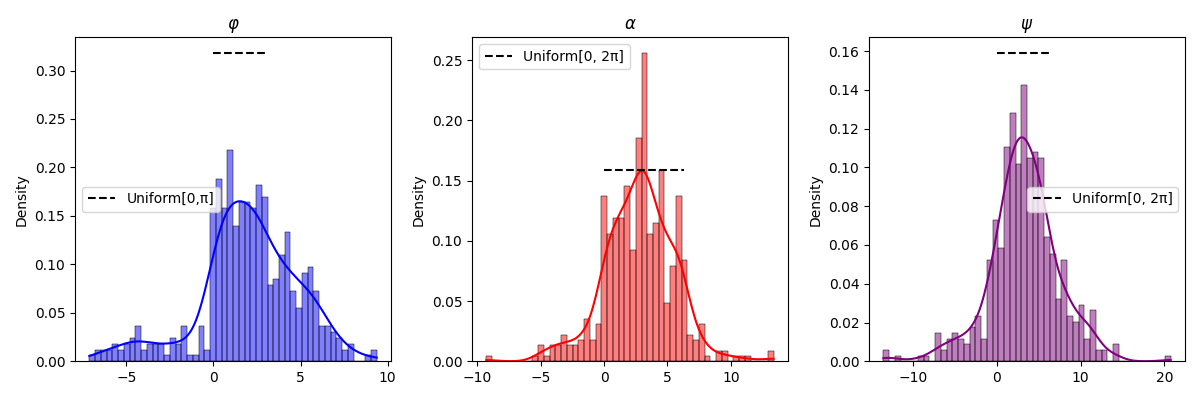
\includegraphics[height=0.35\textwidth]{VariableSelectionPsi/phi_alpha_psi.png}
    \caption{Marginal density of the learned parameters \((\varphi,\alpha,\psi)\)}
    \label{fig:Distributions5.2}
\end{figure}
\begin{figure}[H]
    \centering
    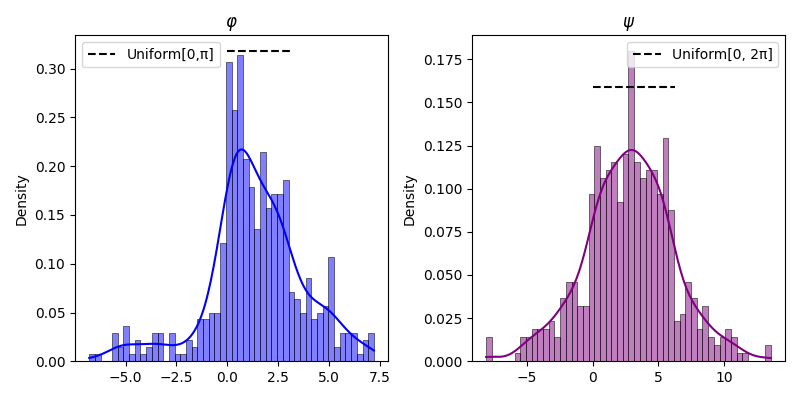
\includegraphics[height=0.35\textwidth]{VariableSelectionPsi/phi_psi.png}
    \caption{Marginal density of the learned parameters \((\varphi,\psi)\)}
    \label{fig:Distributions5.3}
\end{figure}
\begin{figure}[H]
    \centering
    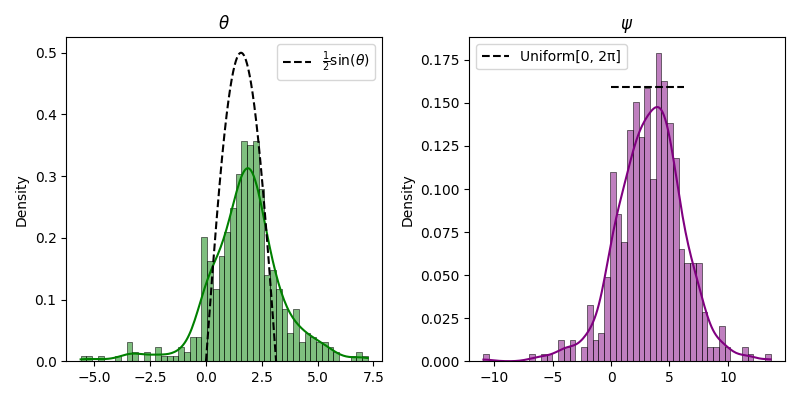
\includegraphics[height=0.35\textwidth]{VariableSelectionPsi/theta_psi.png}
    \caption{Marginal density of the learned parameters \((\theta,\psi)\)}
    \label{fig:Distributions5.4}
\end{figure}
\begin{figure}[H]
    \centering
    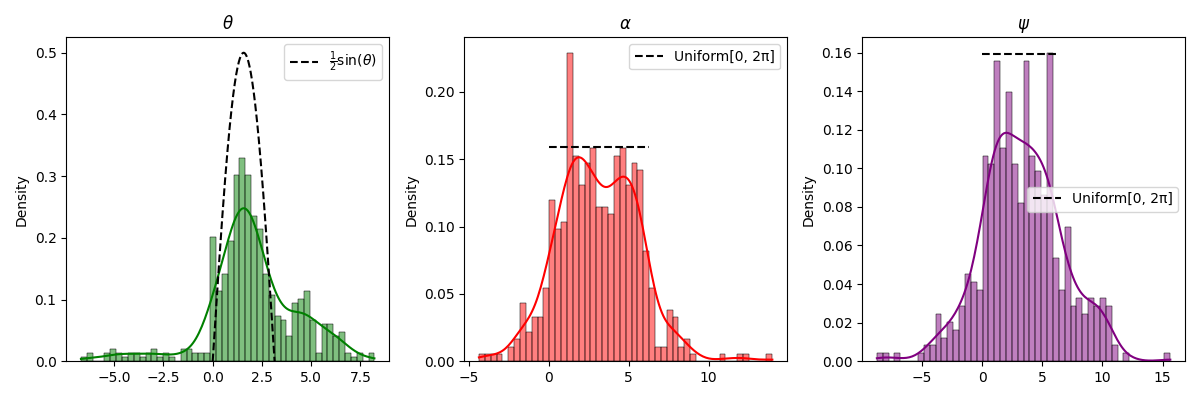
\includegraphics[height=0.35\textwidth]{VariableSelectionPsi/theta_alpha_psi.png}
    \caption{Marginal density of the learned parameters \((\theta,\alpha,\psi)\)}
    \label{fig:Distributions5.6}
\end{figure}
\begin{figure}[H]
    \centering
    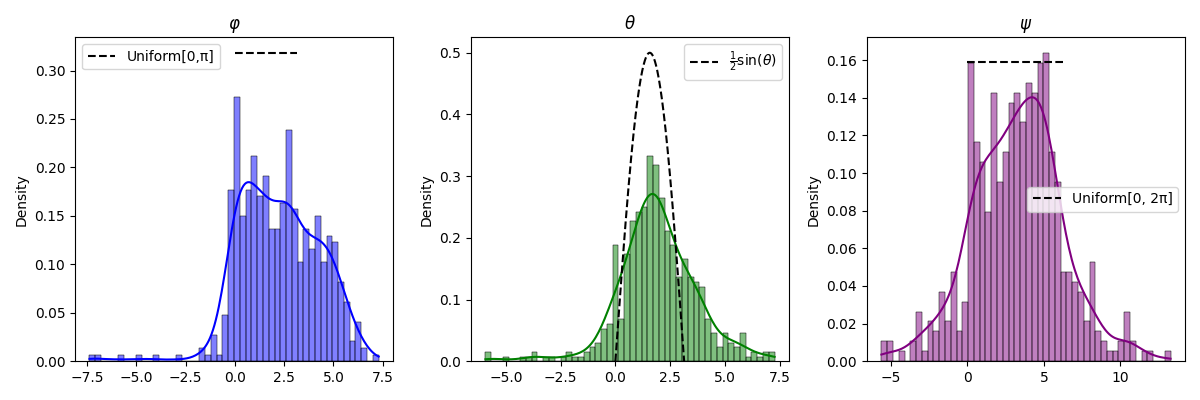
\includegraphics[height=0.35\textwidth]{VariableSelectionPsi/phi_theta_psi.png}
    \caption{Marginal density of the learned parameters \((\varphi,\theta,\psi)\)}
    \label{fig:Distributions5.7}
\end{figure}
\begin{figure}[H]
    \centering
    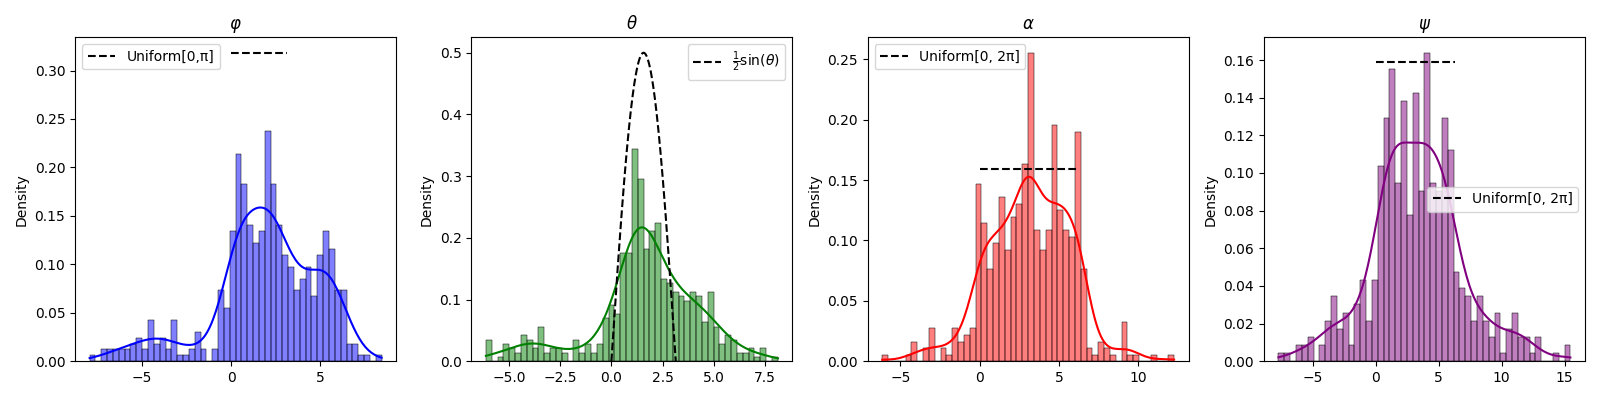
\includegraphics[width=\textwidth]{VariableSelectionPsi/phi_theta_alpha_psi.png}
    \caption{Marginal density of the learned parameters \((\varphi,\theta,\alpha,\psi)\)}
    \label{fig:Distributions5.8}
\end{figure}
Overall, the distribution of the angles appears consistent with the previous case where \(\psi\) was not considered. The distribution of \(\psi\) itself remains pretty consistent across all cases.\\
The distribution of $\alpha$ is the most similar to the base distribution $\mathcal{U}([0,2\pi])$.\\
However, these figures represent only the marginal densities and do not capture the dependencies between parameters.

\subsection{Joint distributions}

\begin{figure}[htbp]
    \centering

    \begin{subfigure}[b]{0.45\textwidth}
        \centering
        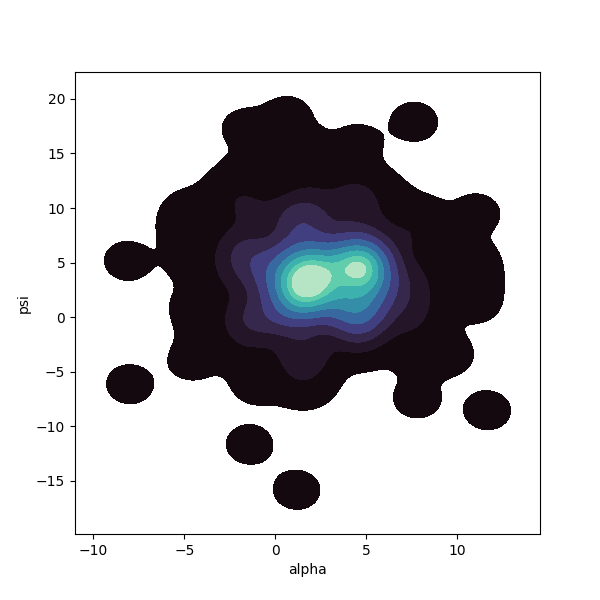
\includegraphics[width=\textwidth]{VariableSelectionPsi/joint_alpha_psi.png}
        \caption{Learned parameters \((\alpha, \psi)\)}
        \label{fig:joint_alpha_psi}
    \end{subfigure}
    \hfill
    \begin{subfigure}[b]{0.45\textwidth}
        \centering
        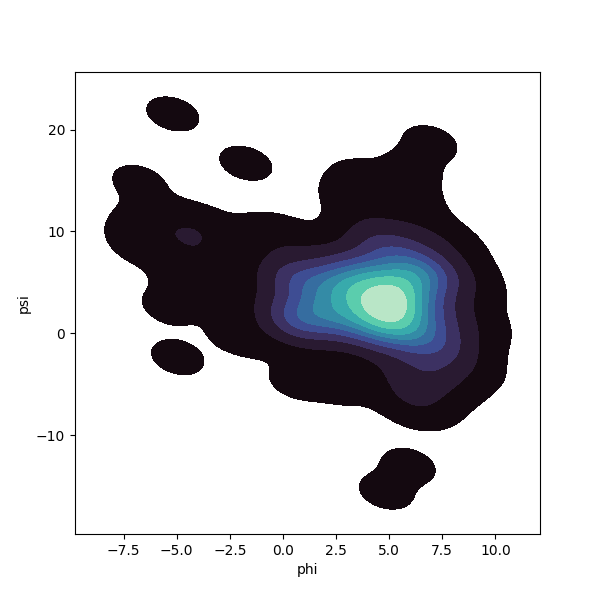
\includegraphics[width=\textwidth]{VariableSelectionPsi/joint_phi_psi.png}
        \caption{Joint distribution of \((\varphi, \psi)\)}
        \label{fig:joint_phi_psi}
    \end{subfigure}

    \vspace{0.5em}

    \begin{subfigure}[b]{0.45\textwidth}
        \centering
        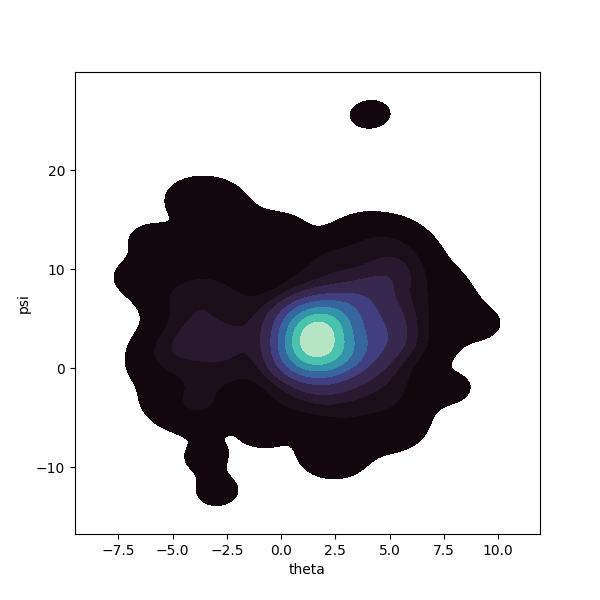
\includegraphics[width=\textwidth]{VariableSelectionPsi/joint_theta_psi.png}
        \caption{Joint distribution of \((\theta, \psi)\)}
        \label{fig:joint_theta_psi}
    \end{subfigure}
    \hfill
    \begin{subfigure}[b]{0.3\textwidth}
        \centering
        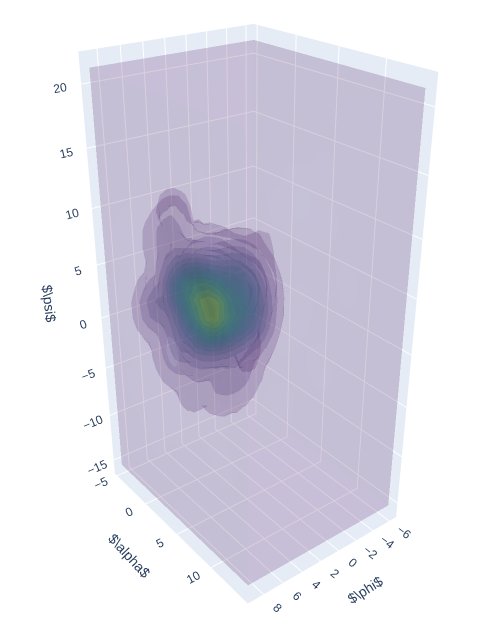
\includegraphics[width=\textwidth]{VariableSelectionPsi/joint3d_phi_alpha_psi.png}
        \caption{Joint distribution of \((\varphi, \theta, \alpha)\)}
        \label{fig:joint3D_phi_alpha_psi}
    \end{subfigure}

    \begin{subfigure}[b]{0.3\textwidth}
        \centering
        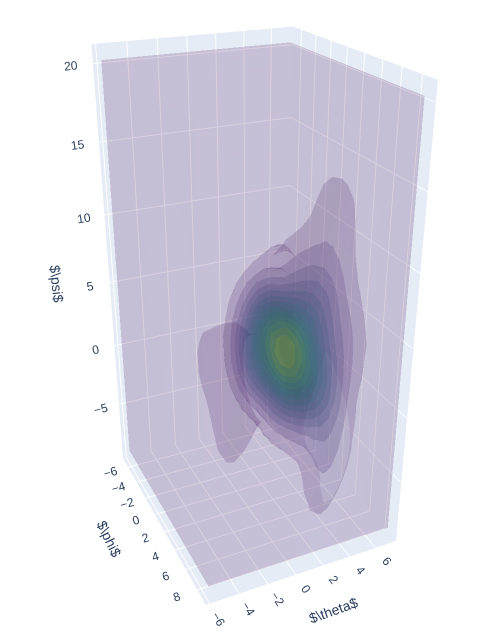
\includegraphics[width=\textwidth]{VariableSelectionPsi/joint3d_phi_theta_psi.png}
        \caption{Joint distribution of \((\theta, \psi)\)}
        \label{fig:joint3D_phi_theta_psi}
    \end{subfigure}
    \hfill
    \begin{subfigure}[b]{0.3\textwidth}
        \centering
        \includegraphics[width=\textwidth]{VariableSelectionPsi/joint3d_theta_alpha_psi.png}
        \caption{Joint distribution of \((\varphi, \theta, \alpha)\)}
        \label{fig:joint3D_theta_alpha_psi}
    \end{subfigure}

    \caption{Joint distributions of parameter combination}
    \label{fig:joint_distributions_psi}

\end{figure}
\newpage
\printbibliography
% \end{comment}

\end{document}